%% Documentation for BOUT++ Drift instability test

\documentclass[12pt]{article}
\usepackage[nofoot]{geometry}
\usepackage{graphicx}
\usepackage{fancyhdr}
\usepackage{subfigure}

\usepackage{listings}
\usepackage{color}
\usepackage{textcomp}
\definecolor{listinggray}{gray}{0.9}
\definecolor{lbcolor}{rgb}{0.95,0.95,0.95}
\lstset{
	backgroundcolor=\color{lbcolor},
        language=C++,
	keywordstyle=\bfseries\ttfamily\color[rgb]{0,0,1},
	identifierstyle=\ttfamily,
	commentstyle=\color[rgb]{0.133,0.545,0.133},
	stringstyle=\ttfamily\color[rgb]{0.627,0.126,0.941},
	showstringspaces=false,
	basicstyle=\small,
	numberstyle=\footnotesize,
	numbers=left,
	stepnumber=1,
	numbersep=10pt,
	tabsize=2,
	breaklines=true,
	prebreak = \raisebox{0ex}[0ex][0ex]{\ensuremath{\hookleftarrow}},
	breakatwhitespace=false,
	aboveskip={1.5\baselineskip},
        columns=fixed,
        upquote=true,
        extendedchars=true,
        morekeywords={Field2D,Field3D,Vector2D,Vector3D,real,FieldGroup},
}

%% Modify margins
\addtolength{\oddsidemargin}{-.25in}
\addtolength{\evensidemargin}{-.25in}
\addtolength{\textwidth}{0.5in}
\addtolength{\textheight}{0.25in}
%% SET HEADERS AND FOOTERS

\pagestyle{fancy}
\fancyfoot{}
\renewcommand{\sectionmark}[1]{         % Lower case Section marker style
  \markright{\thesection.\ #1}}
\fancyhead[LE,RO]{\bfseries\thepage}    % Page number (boldface) in left on even
                                        % pages and right on odd pages 
\renewcommand{\headrulewidth}{0.3pt}

%% commands for boxes with important notes
\newlength{\notewidth}
\addtolength{\notewidth}{\textwidth}
\addtolength{\notewidth}{-3.\parindent}
\newcommand{\note}[1]{
\fbox{
\begin{minipage}{\notewidth}
{\bf NOTE}: #1
\end{minipage}
}}

\newcommand{\noun}[1]{\textsc{#1}}
\newcommand{\deriv}[2]{\ensuremath{\frac{\partial #1}{\partial #2}}}
\newcommand{\code}[1]{\texttt{#1}}
\newcommand{\file}[1]{\texttt{\bf #1}}
\newcommand{\pow}{\ensuremath{\wedge}}
\newcommand{\poweq}{\ensuremath{\wedge =} }

%\newcommand{\deriv}[2]{\ensuremath{\frac{\partial #1}{\partial #2}}}
\newcommand{\apar}{\ensuremath{A_{||}}}
\newcommand{\hthe}{\ensuremath{h_\theta}}
\newcommand{\Bp}{\ensuremath{B_\theta}}
\newcommand{\Bt}{\ensuremath{B_\zeta}}
\newcommand{\Vec}[1]{\ensuremath{\mathbf{#1}}}
\newcommand{\bvec}{\Vec{b}}
\newcommand{\kvec}{\Vec{\kappa}}
\newcommand{\bxk}{\bvec_0\times\kvec_0\cdot\nabla}
\newcommand{\Bvec}{\Vec{B}}
\newcommand{\Bbar}{\overline{B}}
\newcommand{\Lbar}{\overline{L}}
\newcommand{\Tbar}{\overline{T}}
\newcommand{\Jvec}{\Vec{J}}
\newcommand{\Jpar}{J_{||}}
\newcommand{\delp}{\nabla_\perp^2}
\newcommand{\Div}[1]{\ensuremath{\nabla\cdot #1 }}
\newcommand{\Curl}[1]{\ensuremath{\nabla\times #1 }}
\newcommand{\rbpsq}{\ensuremath{\left(R\Bp\right)^2}}

\begin{document}

\title{Resistive drift-wave instability test}
\author{M.Umansky, LLNL, \\
B.Dudson, University of York}
\maketitle

\tableofcontents

\section{Introduction}

A drift-wave is a wave which exists in a plasma wherever there is a pressure
gradient \cite{hazeltine-2003}.
Without dissipation, fluctuations in density $n$ and electrostatic
potential $\phi$ are in phase
so there is no transport of plasma and the wave amplitude does not grow.
Dissipation, in this case resistivity, introduces a phase-shift
between $n$ and $\phi$ and hence transport of plasma and growth of the mode.
Since all that is required for radial transport is a pressure gradient
and some form of dissipation (in the absence of magnetic shear), this is often called the ``universal''
instability. 
Because the growth of the resistive drift-wave instability is sensitive to
phase shifts, this test checks how accurately this phase is simulated.

The equations solved are for the density $n$, and vorticity
$\omega = n_0\mathbf{b}\cdot\Curl{\mathbf{v}}$.
The simulation is electrostatic, and the zero electron mass approximation
is used to obtain the parallel current $j_{||}$. All quantities with a '$0$'
subscript are equilibrium and not evolved.
\begin{eqnarray*}
\deriv{n}{t} &=& -\mathbf{V}_E\cdot\nabla n_0 \\
\deriv{\omega}{t} &=& \frac{B_0^2}{m_i}\nabla_{||}j_{||} \\
\mathbf{V}_E &=& \frac{1}{B_0}\mathbf{b}_0\times\nabla_\perp\phi \\
\nabla_\perp^2\phi &=& \omega/n_0 \\
j_{||} &=& \sigma_{||}\left(T_0\partial_{||}n - n_0\partial_{||}\phi\right)
\end{eqnarray*}
The simulation domain is a cylindrical annulus with radius $R = 5.4$~m, radial width $6$~cm and constant
density scale-length $L_N = 4.5$~m. This is a 2D periodic simulation domain, but since perpendicular
wavenumber is fixed in a given simulation, the simulation is effectively 1D. Radial boundary conditions are
zero-gradient vorticity and density, and $\phi = 0$. 
Numerical methods used were $4^{th}$-order central differencing, and $3^{rd}$-order WENO for advection terms
on a 32x32 grid. A relative tolerance of \code{1.0e-7}, and absolute tolerance of \code{1.0e-12} were specified.

The analytic dispersion relation is $\left(\omega - \omega_*\right)i\sigma_{||} + \omega^2 = 0$, with
diamagnetic frequency $\omega_* = k T_{e0} / L_N$ \cite{umansky-2008-tests}.

\begin{figure}[htbp!]
\centering
\subfigure[Growth rate]{
  \label{fig:drift_imag}
  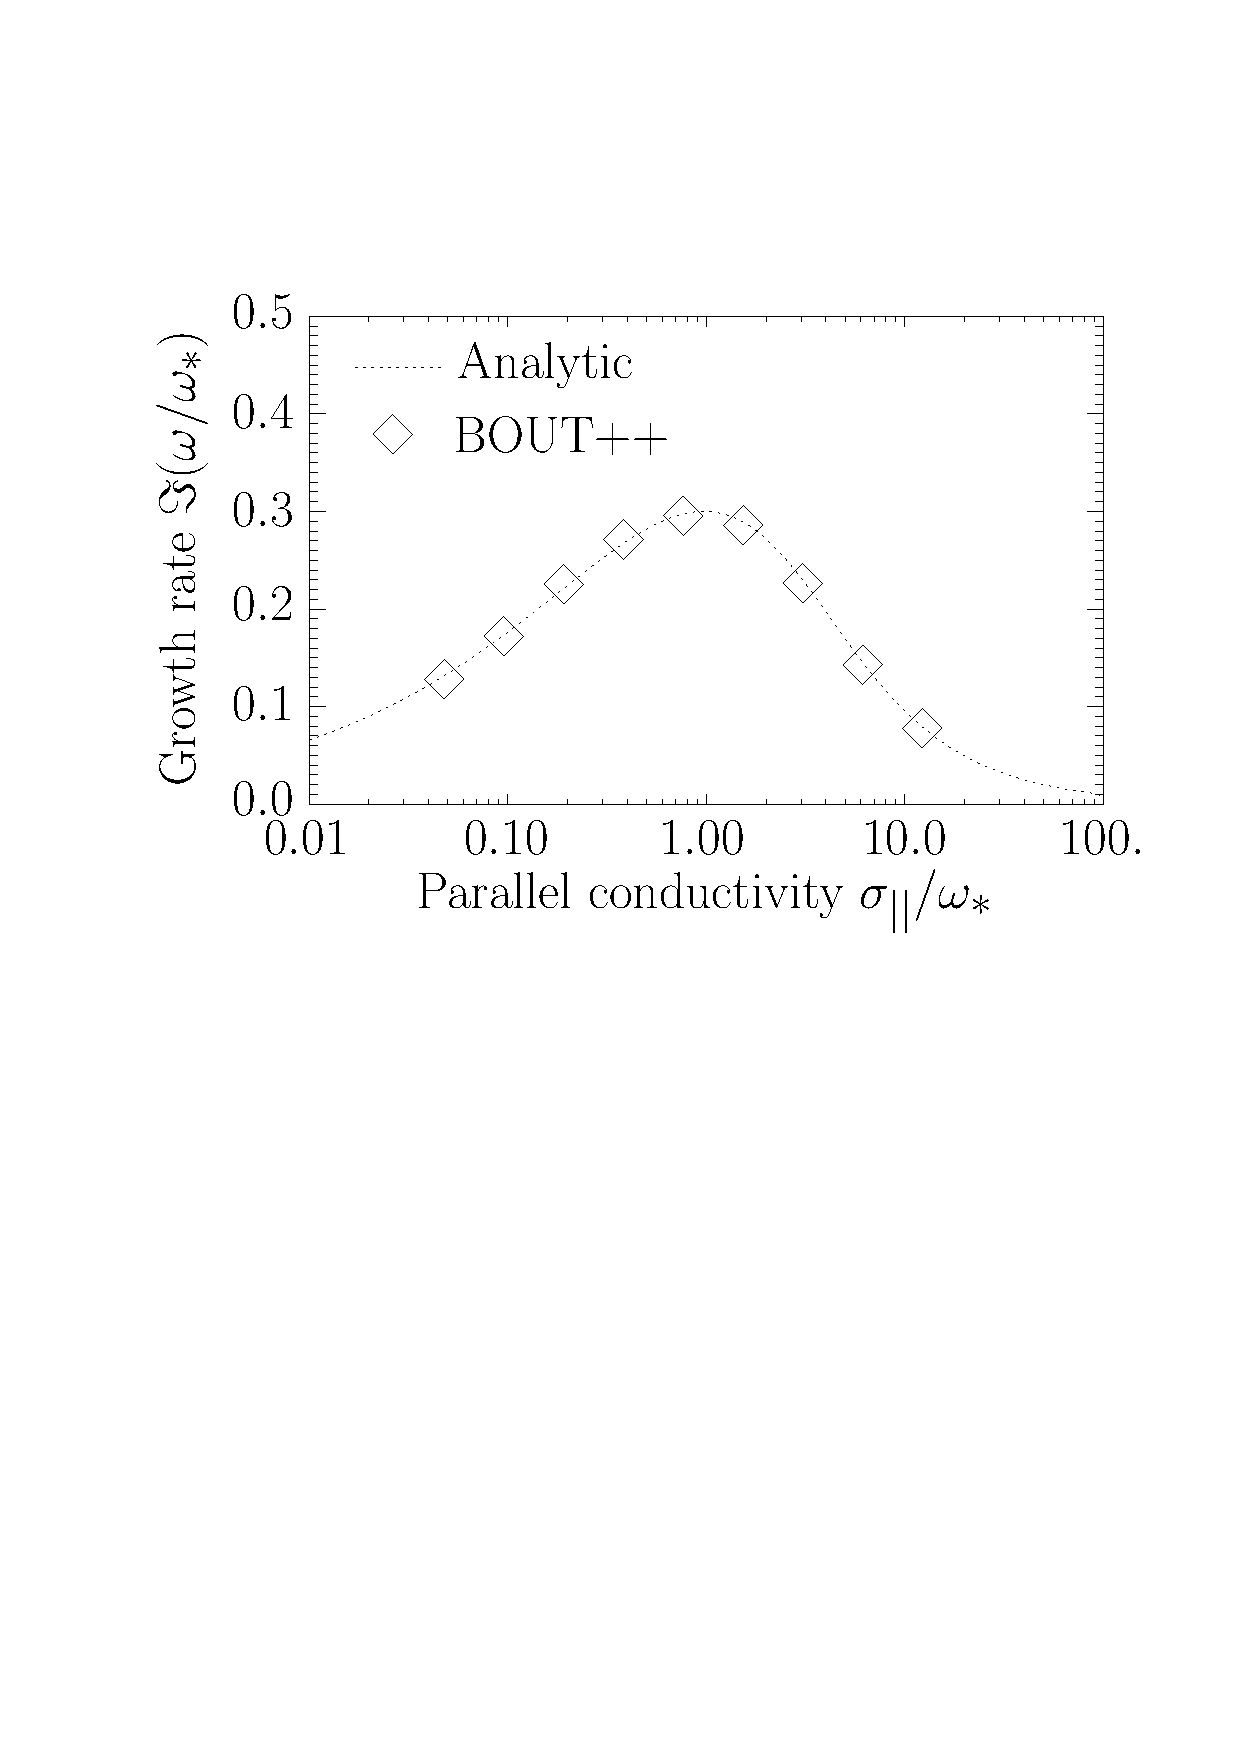
\includegraphics[scale=0.35]{drift_growth.pdf}
}
\subfigure[Real Frequency]{
  \label{fig:drift_real}
  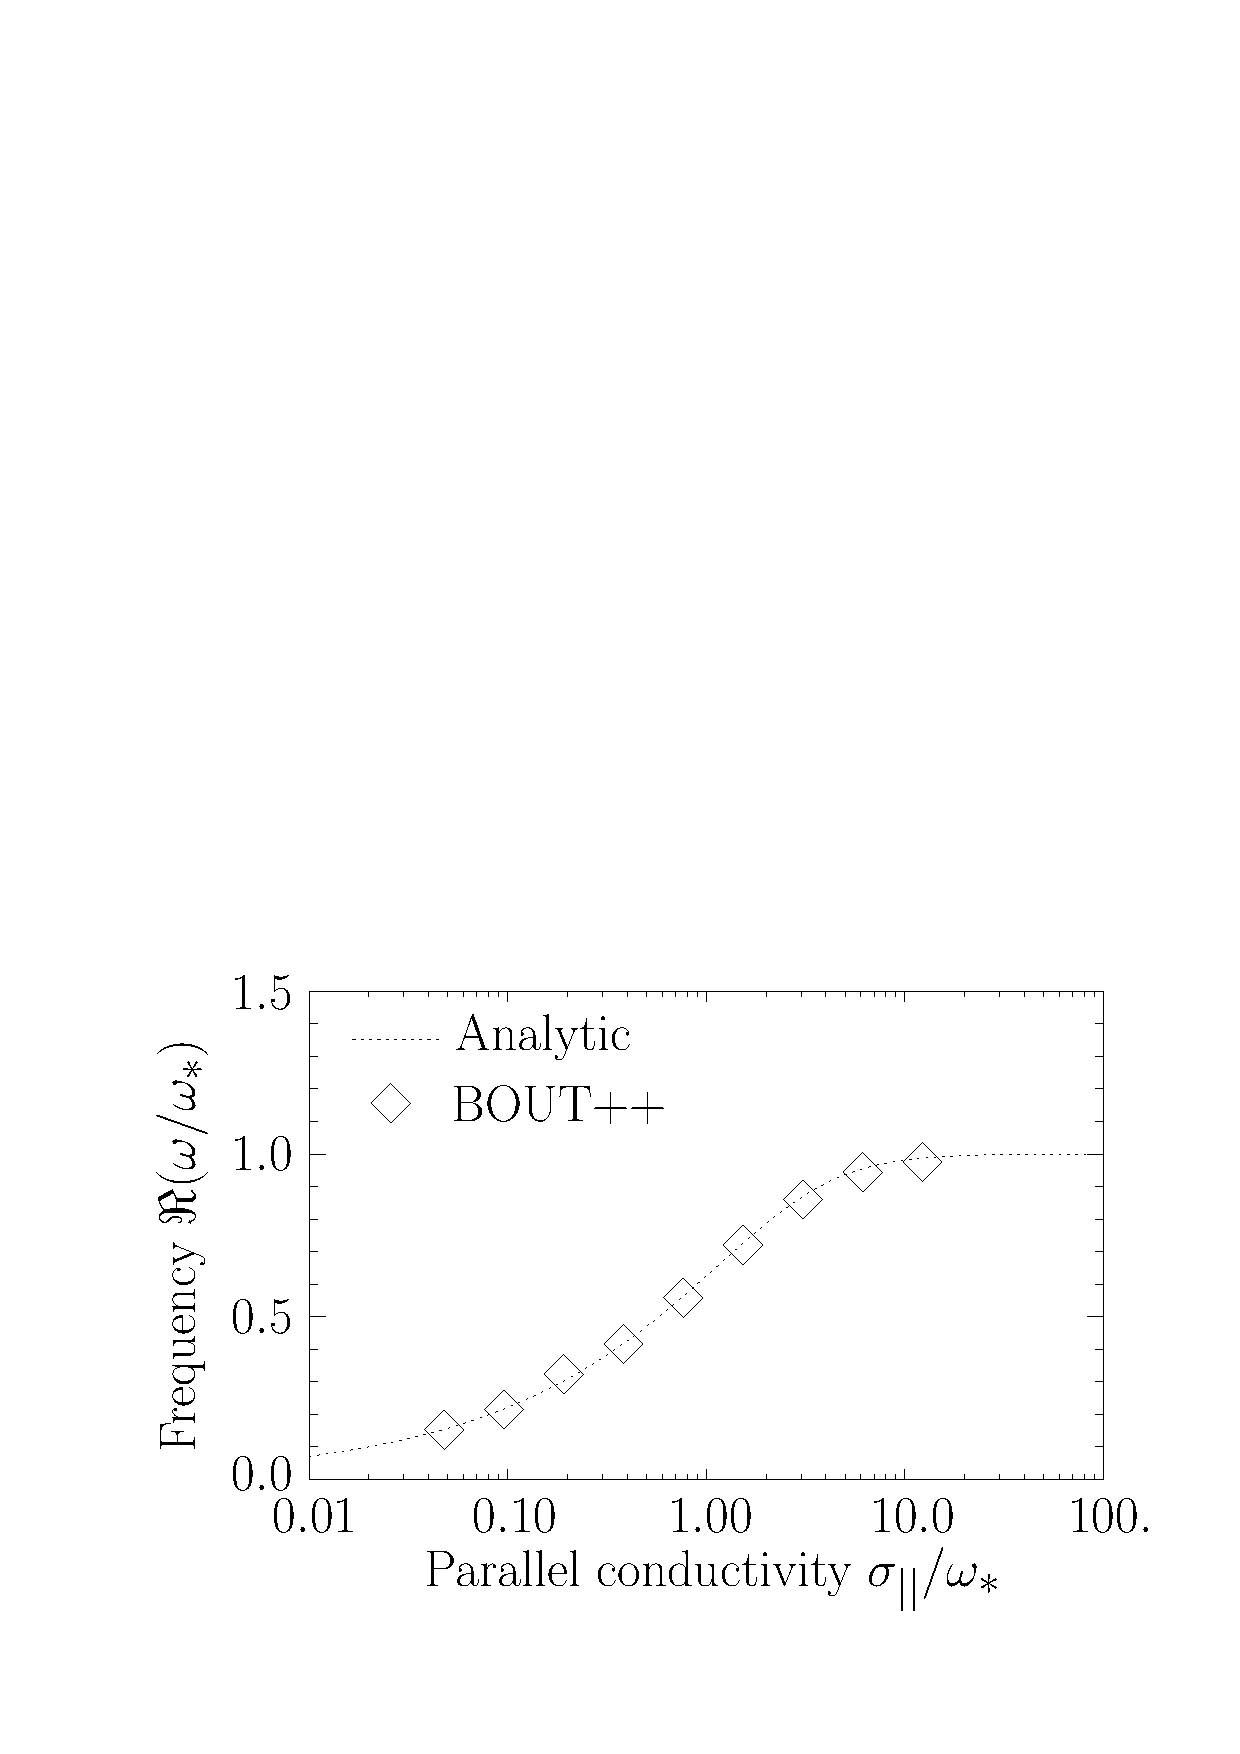
\includegraphics[scale=0.35]{drift_freq.pdf}
}
\end{figure}

\section{Input grid}



\section{Options file}

The file BOUT.inp is used for all runs here, with the 
Zeff value being changed each time.

\section{Code}



\bibliography{drift_instability}
\bibliographystyle{unsrt}
\end{document}
